\chapter{Implementation}

%The implementation should look at any issues you encountered as you tried to implement your design. During the work, you might have found that elements of your design were unnecessary or overly complex; perhaps third party libraries were available that simplified some of the functions that you intended to implement. If things were easier in some areas, then how did you adapt your project to take account of your findings?
%
%It is more likely that things were more complex than you first thought. In particular, were there any problems or difficulties that you found during implementation that you had to address? Did such problems simply delay you or were they more significant?

%You can conclude this section by reviewing the end of the implementation stage against the planned requirements. 
	
\section{Data Downloading}
\label{sec:imp_data_download}
%discuss data downloader implementation, discussing file name pattern and challenges with that, as well as %difficulties with storage as dataset is large
One of the first parts of the system to be implemented was the Data Downloader. This was done first in order to get the full dataset downloaded as fast as possible, and also as a form of Python practice.

As mentioned in Section \ref{sec:des_data_downloader}, the files that needed to be downloaded from the online archive had a specific format that made finding all the files required easier. Each series had a specific URL, and all files for that series would be stored as children of that URL in zip files. The naming pattern for the files was as follows:

\textbf{S\emph{s}V\emph{vvvv}P\emph{p}.zip}

where \emph{s} is the series from 1 to 6, \emph{vvvv} is 4 digits representing the volume of the series, starting at 0001, the max value depending on which series it is a part of, and \emph{p} is a part number, as some files were split into multiple parts. This could be zero, if the file is not split, or a one or two if it has been split. For instance \emph{S6V0141P1.zip} would represent the \emph{1st} part of the \emph{141st} volume in series \emph{6}.

There was one difference to this pattern, discovered during development. Series 5 of Hansard was separated into records for the \emph{House of Commons} and the \emph{House of Lords}. For these, the letter \emph{C} or \emph{L} was added before the V to differentiate the two series. Afterwards, series 6 also contained the letter \emph{C} to show that it was also only for the house of commons. So, for Series 6, volume 141, part 1, the file format would actually be \emph{S6CV0141P1.zip}.

\subsection{Online Connection}
\label{sec:imp_online_connect}
Python has a commonly used library for HTTP connections called \href{http://docs.python-requests.org/en/master/}{\emph{Requests}}. It provides an API (\emph{Application Programming Interface}) allowing easy connection to a provided URL, simply by providing a URL. Using this API, the downloader can check to see if a file exists, using the code snippet Algorithm \ref{lst:downloader_snippet}.

\begin{lstlisting}[float=ht,
				   caption={Snippet of the Downloader Code},
				   label={lst:downloader_snippet}]
for i in range(0, 100):  # change depending on how many files it looks like exist
    for j in range(0, 4):  # just to make sure. Not seen any files with P3 at the end but you never know
        temp_url = '{}{}/{}'.format(url_base, url_add[series-1], file_name_format.format(series, i, j))
        print("Checking: {}".format(file_name_format.format(series, i, j)))
        r = requests.get(temp_url)
        status = r.headers['content-type']
# if the zip file exists, the type will appear like this:
        if status == 'application/zip; charset=utf-8':  
            print("FILE FOUND")
            zip_ref = zipfile.ZipFile(io.BytesIO(r.content))
            zip_ref.extractall(save_loc)  # extract the file
            zip_ref.close()

        else:  # if the zip file doesn't exist an error page is returned instead
            print("FILE NOT FOUND")
\end{lstlisting}

Effectively, this code snippet loops through the files following the described pattern, and gets the status of the constructed URL. the \emph{header} part returns a string that describes the type of file returned, as if the file does not exist, it still returns a 404 error page rather than not returning anything. If the file does exist, however, it returns a string that says it is a ZIP file type (\emph{"application/zip"}).

If the file does exist, the downloader also makes use of a library called \emph{zipfile}, which allows it to handle zip files internally. It can then extract the data file from the compressed zip file, and save it to the designated directory on the local machine.

\subsection{Dataset Size}
\label{sec:imp_dataset_size}

The total Historical Hansard Dataset that was downloaded by the project is \emph{14.4GB}, and consists of \emph{2503} files, demonstrating the need for the automated downloading. Due to this size, the dataset could not be saved to the University file system, and so was saved to an external hard drive instead. This meant that some parts of the later development were slowed due to the USB 3 connection used by said hard drive. 

\section{Data Parsing}
\label{sec:imp_data_parse}
%discuss experimentation with how to extract data from original dataset. discuss change made to format of parsed data part way through to make it easier to annoate.
During development of the system, the Data Parser and associated methods were where the most time was spent, due to many unforeseen complications.
 
\subsection{Name Recognition and Disambiguation}
\label{sec:imp_name_disamb}
%here discuss difficulties in name disambiguation. discuss attempted methods of using NLTKs named entity %thing and the implemented regex solution. Discuss how the regex solution only works because the names are %presented in a predicable pattern, and would not be valid outside of this dataset
Part of the difficulty in parsing the data accurately was ensuring speech spoken by one person was always attributed to that person, even though the references to that person may use multiple versions of their name. In order to correctly attribute speech to the speaker, without duplicating references to them, a method of NLP called "Name Disambiguation" must be employed.

Name Disambiguation is the method of identifying proper names in text, and recognizing when two proper names refer to the same subject or person.\cite{Wacholder1997} Many difficulties exist for such a task, as names can come in many forms. Proper nouns can often refer to multiple things. \emph{Johnson and Sons} might refer to a business by that name; two people with the surnames \emph{Johnson} and \emph{Sons}; or someone called \emph{Johnson} and their male children. In this example, the context of the sentence the name appears in may provide clues to which it is, but this is not always an option.

Thankfully, this project only needs to be able to recognize the names of the Members of Parliament mentioned in the Hansard Dataset, which displays more structure in the way it names people than normal human speech would.

\begin{figure}[ht]
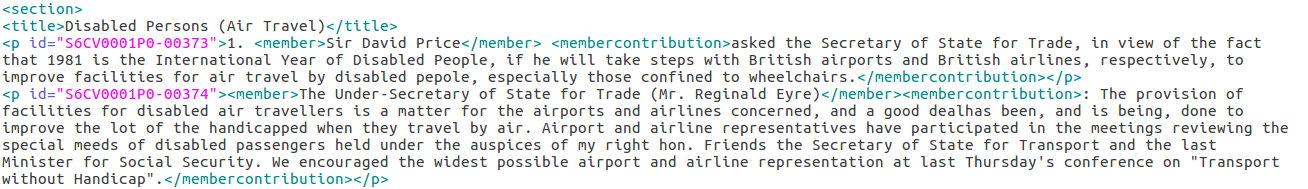
\includegraphics[width=\textwidth]{dataset_name_example}
\caption{An example from the original dataset, showing that names exist only within \emph{member} tags}
\label{fig:dataset_name_example}
\end{figure}

As can be seen in Figure \ref{fig:dataset_name_example}, the names needed for this project are always contained within a \emph{member} tag. They still contain the full job title at times, but this means that the area the project needs to look for a name is well defined. It can be guaranteed that, if a member tag is encountered, it will contain the name of the member.

The first attempted method of extracting the name from the \emph{member} tag was using the \emph{Named Entity Chunker} from NLTK, which is designed to extract the Named Entities from a piece of text and return them in a list. Using this, the name could be extracted, potentially along with other parts of the title (\emph{The Under-Secretary of State for Trade (Mr. Reginald Eyre)} would be returned as a list of two names, \emph{State for Trade} and \emph{Mr. Reginald Eyre}). The thought was that the actual name desired could be chosen from that list by looking for the item that started with an Honorific, such as \emph{Mr.}, \emph{Mrs.} and other such titles. However, the Named Entity Chunker did not work consistently enough for it to be a viable solution for the name extractor, as it often separated the honorific from the name. Due to this, it could not be reliably used to extract the names, because there was no way to recognize, when it returned multiple names, which referred to the actual person, and which was a part of their job title.

The second method attempted, which was the one settled on for the project, was the use of Regular Expressions to search for the expected name format. This method relies on a lot of assumptions about the organization of the original dataset, but appears to be good enough for the current dataset. The assumptions are as follows:
\begin{itemize}
	\item All Names start with an Honorific (Mr, Mrs, Sir etc)
	\item All Names End with a Surname
	\item The first time a person is seen, their full name and job title, if relevant, are presented
\end{itemize}

Following these assumptions, Regular Expressions could be used to find the honorific at the start of the name, then get everything following it until either the end of the text, or a piece of punctuation not commonly used in names, such as a bracket.
\begin{figure}[ht]
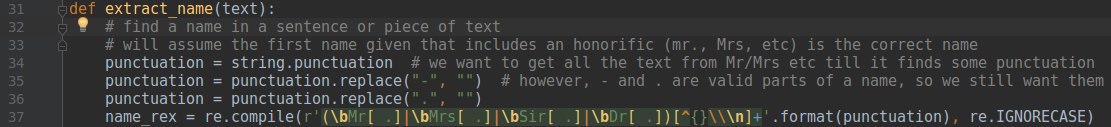
\includegraphics[width=\textwidth]{extract_name_code_example}
\caption{Extract of code from the Name Extractor Method.}
\label{fig:name_extract_code}
\end{figure}

Figure \ref{fig:name_extract_code} shows the regular expression used to extract a name from a piece of text. It searches for an Honorific to start it off, either \emph{Mr}, \emph{Mrs}, \emph{Dr} or \emph{Sir}. Once it find one of these honorifics it gets everything after it that is not a punctuation mark listed, as shown by the \verb|[^{}\\\n]+| part at the end of the regular expression. The \verb|{}| brackets in that part are replaced with the string called \emph{punctuation}, generated by the string package, so that it becomes a list of all punctuation possible, including new line characters.  

\subsection{Name Matching}
\label{sec:imp_name_match}
Once names can be reliably extracted from the source text, a method of comparing two names to see if they referred to the same person had to be developed. This becomes a very complicated issue, simplified only slightly by the assumptions mentioned previously.

\begin{table}[ht!]
\centering
\begin{tabular}{|c c c|}
Name One & Name Two & Same Person? \\
\hline
Mr. Adam Neaves  & Mr. Adam Neaves & True \\
Mr. A. Neaves    & Mr. Adam Neaves & True \\
Dr. Adam Neaves  & Mr. Adam Neaves & False, wrong Honorific \\
Mr. B. Neaves    & Mr. Adam Neaves & False, wrong First Name \\
Adam Neaves      & Mr. Adam Neaves & True, despite missing honorific \\
Mr. A. B. Neaves & Mr. Adam Neaves & True, though slightly ambiguous \\
Mr. A. B. Neaves & Mr. Neaves      & True, though again ambiguous    \\
\end{tabular}
\caption{Table showing the different ways names might or might not refer to the same person}
\label{tbl:name_match}
\end{table}

For instance, as shown in Table \ref{tbl:name_match}, first names might be shortened to just an initial, or even fully removed. Honorifics are not guaranteed to be present, but are very important if they are, as two different names may differ from only that.

The implemented algorithm for this project follows the same assumptions mentioned in Section \ref{sec:imp_name_disamb}, and is designed to allow for some false negatives (wherein two names that \emph{do} refer to the same person might not appear as the same person) to avoid any false positives at all. This is because it was desicided that speech accidentally attributed to the wrong person would be worse than accidentally having duplicate references to a person, since a human reader can likely see the connection between \emph{Mr. Adam Neaves} and \emph{Mr. A Neaves}, but there would be no way for them to know that some speech was attributed to the wrong person. The basic algorithm implemented is as shown in Algorithm \ref{lst:name_match}.
\begin{lstlisting}[float=ht,
				   caption={Pseudocode representing the name matching method},
				   label={lst:name_match}]
if BOTH NAMES ARE EXACTLY THE SAME
	return True
SPLIT BOTH NAMES INTO COMPONENT WORDS
for EACH NAME
	if NAME CONTAINS 3 WORDS
		FIRST WORD IS HONORIFIC
		SECOND WORD IS FORENAME
		THIRD WORD IS SURNAME
	else
		FIRST WORD IS HONORIFIC
		LAST WORD IS SURNAME
		IGNORE ANYTHING ELSE
if FORENAME ONE and FORENAME TWO BOTH EXIST
	FORNAME_MATCH = FORNAME ONE == FORNAME TWO
else
	FORNAME_MATCH = True
SURNAME_MATCH = SURNAME ONE == SURNAME TWO
HONORIFIC_MATCH = HONORIFC ONE == HONORIFIC TWO

if SURNAME_MATCH, HONORIFIC_MATCH and FORENAME_MATCH ARE True
	return true
else return False
\end{lstlisting}

This method does work so long as the assumptions in Section \ref{sec:imp_name_disamb} hold true. It would not be a valid method of matching names in a more generalized setting where the formatting and appearance of names would vary wildly.

\subsection{Saving Parsed Data}
\label{sec:imp_saving_pased_data}

The parser would save the information extracted from the original data files in newly created XML files. Due to some character use in the original dataset, these files had to be opened by the Python script in \emph{Binary Mode}, meaning it would treat the data as bytes of data rather than strings of text. Due to this, when editing a file, the Parser could not simply append data to the file, but rather would have to overwrite the whole file. Therefore, when editing a parsed file to add more data to it, it was necessary to load the whole file into memory, edit that data, then overwrite the whole set of data to the XML file again.
This was one of the main reasons for the change in data structure part way through implementation described in Section \ref{sec:des_parsed_data}. When the Parser was designed to write an entire series to a single file, it would take an increasingly long time to read the whole file into memory, then save the data back to the file once modified. At the start of a session of parsing, it would take an average of \emph{3 seconds} to parse the first file from the original dataset, but as it parsed more of a series, each additional file would increase the time it took substantially. Table \ref{tbl:original_parse_time} shows the time taken on a subset of one series.

\begin{table}[ht!]
\centering
\begin{tabular}{c | c}
	\textbf{Source Data File Number} & \textbf{Time to Parse (s)} \\
	\hline
	0001 & 2.564   \\
	0002 & 3.245   \\
	0003 & 4.632   \\
	...  & ...     \\
	0250 & 302.452 \\
	0251 & 306.321 \\

\end{tabular}
\caption{Excerpt from the log of the original parser parsing Series 6, showing time it took to parse each file}
\label{tbl:original_parse_time}
\end{table}

As can be seen, the additional time taken for each file meant that, in order to parse an entire series, the parser would take up to a few hours to finish. Additionally, as the large files had to be loaded into memory in order for them to be edited, the Parser would use a large amount of RAM, at one point during development getting up to around 10GB of RAM used.

Therefore, instead of saving an entire series worth of data to a single file, the decision was made to split the files by date instead. The parser would search through each file, creating a new file for each date it encountered, so that everything that was debated on that date would be saved to that file. This meant that the parsed data files were smaller, and meant that the data that had to be loaded into memory in order to be modified was much smaller, so the Parser didn't use anywhere near as much RAM. It also meant that the time taken per file parsed was constant, and only depended on the size of the original file, rather than the number of files already parsed. This was a much better solution, and also encouraged a better design for the parsed data layout, as described in Section \ref{sec:des_parsed_data}.

Additionally, though the parsed data consisted of more files than the original dataset, the set of parsed data was usually smaller than the original, due to the parser stripping out unneeded information. The exact values can be seen in Table \ref{tbl:parsed_data_size_comp}

\begin{table}[ht!]
\centering
\begin{tabular}{r || l | l || l | l}
	& \multicolumn{2}{|c||}{\textbf{Original Dataset}} & \multicolumn{2}{|c}{\textbf{Parsed Dataset}}\\
	\hline
	\textbf{Series} & \textbf{Size (GB)} & \textbf{Number Of Files} & \textbf{Size (GB)} & \textbf{Number Of Files}\\
	\hline
	\hline
	1 & 0.0943 & 27   & 0.0691 & 1245\\
	2 & 0.0877 & 22   & 0.0755 & 926\\
	3 & 1.4    & 305  & 1.2    & 6888\\
	4 & 0.6461 & 133  & 0.3842 & 1551\\
	5 & 5.5    & 900  & 3.4    & 9742\\
	6 & 3.5    & 446  & 1.7    & 3745\\
\end{tabular}
\caption{Size comparison between the Original Hansard Dataset and the Parsed Dataset generated by the Parser}
\label{tbl:parsed_data_size_comp}
\end{table}

\section{Manual Annotation Tool}
\label{sec:imp_manual_annotate}

With all the source data successfully parsed, the Manual Annotation Tool (MAT) could be developed to use that data to create the training dataset discussed in Section \ref{sec:des_anotate_data}.

Originally, as discussed in Section \ref{sec:des_annotation_tool}, this tool was designed to print everything a single MP said about a particular topic, but this often meant far too much text was printed on the screen at any one time. Additionally, this tool was also designed to allow the user to edit the name of the MP, or the topic, in case of typos in the text. However, it was felt that the tool was overcomplicated by this added functionality.

Instead, the Annotation tool now only displays one sentence at a time, and allows the user to quickly annotate it by entering only a single character, as shown in Figure \ref{fig:annotate_screenshot}. That helped to speed up the process of annotating data, which was already a lengthy process, in order to create the training set needed for the Artificial Intelligence Algorithm.

\begin{figure}[ht]
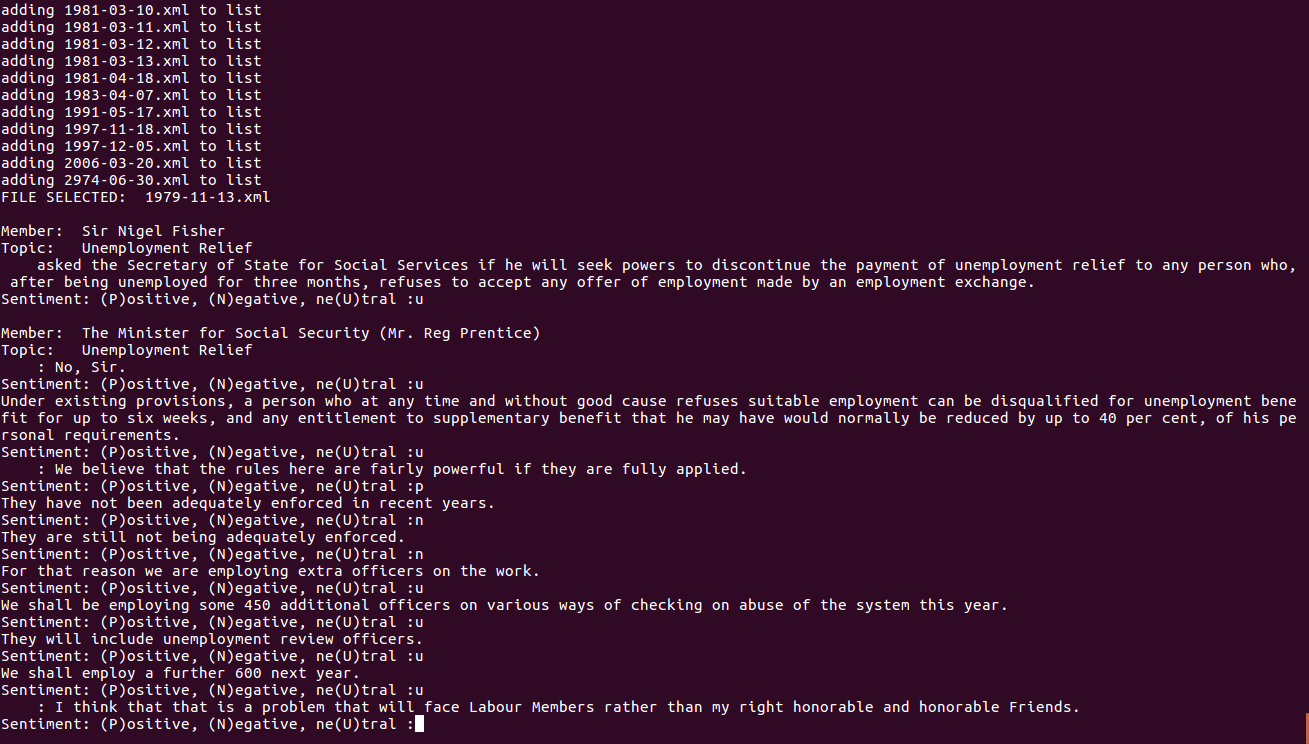
\includegraphics[width=\textwidth]{annotate_screenshot}
\caption{Screenshot from the Annotation Tool running on the Command Line}
\label{fig:annotate_screenshot}
\end{figure}

\subsection{Sentence Splitting}
\label{sec:imp_sentence_split}
% discuss dificulties getting NLTKs sentence tokenizer to work with the data
An important part of the update to the Annotation tool was the ability to separate a block of text by sentence. This is not as simple as it sounds, as the text can't just be split whenever a \emph{"."} character is encountered, as there are acronyms in some of the text, and some sentences might include a quote with a period in it, which must be included in the sentence structure.

NLTK does include a sentence tokenizer as a part of it's library. This method is designed to receive a block of text as an input, and returns an array of sentences, split by the tokenizer. However, this function did not work perfectly for the data used, as there were a few special cases, such as typos, that the tokenizer provided was not prepared for. In order to improve the quality of the splitting, some parts of the text had to be modified, so that the tokenizer would either stop seeing sentence boundaries where there were none, or missing sentence boundaries. These changes were as follows:

\begin{itemize}
	\item The word \emph{Honorable} had to replace the word \emph{Hon.}, which was often used as a short hand. NLTK's tokenizer did not recognise this and therefore split sentences on the period of that word.
	\item If the Members of Parliament discussed some form of percentage, it was commonly refered to as \emph{per cent.}, which the sentence tokenizer saw as the end of a sentence due to the period. This was replaced with the word \emph{percent}.
	\item The Parser would strip out any new line characters from text before saving it. This, combined with issues from the original data, meant that when a sentence ended, it was common for it to miss out any sort of space between the period that marked the end of the sentence, and the start of the next sentence. Due to this missing space, the tokenizer wouldn't realize that it was supposed to be a sentence boundary and therefore wouldn't split the text. Regular expressions were used to find areas of text where it looked like this had occurred, and would input the space.
\end{itemize}
 
Following these corrections, the code that performed the sentence splitting became that shown in Algorithm \ref{lst:sentence_split}.

\begin{lstlisting}[float=ht,
				   caption={Sentence Splitting method, with included regular expressions},
				   label={lst:sentence_split}]
def sentence_split(text):
	# because NLTK's sentence tokenizer recognises hon.
	# as the end of a sentence, unlike mr. or mrs., we need to
    # replace that with something it can handle    
    regex_hon = re.compile(r'\bhon\.', re.IGNORECASE)
    regex_percent = re.compile(r'\bper cent\.', re.IGNORECASE)
    # some sentences are missing the space. Add it back in.
    regex_sentence_end = re.compile(r'([a-z])\.([A-Z])') 
    text = re.sub(regex_hon, "honorable", text)
    text = re.sub(regex_percent, "percent", text)
    text = re.sub(regex_sentence_end, r'\1. \2', text)
    text = text.replace('\n', ' ')
    # once all regex is done, send text to the tokenizer
    return sent_tokenize(text)
\end{lstlisting}

As can be seen by this function, each replacement required is handled using regular expressions, which allow it to quickly search the whole text given to it for these issues described, and fix them, before the text is then sent to the sentence tokenizer of NLTK to be split into an array. This method works well, though it is not the most maintainable, as it would have an issue if many more special cases were found.

\section{Sentiment Analyzer}
\label{sec:imp_sentiment_analyzer}

The sentiment analysis tool builds upon the methods provided by NLTK. The tool provides a method to train the AI algorithm, and also methods to analyze the sentiment for sentences and paragraphs using the trained algorithm. Though NLTK does provide a sentiment analyzer as part of its package, this was a pre-trained algorithm that had been trained on a Movie Review corpus. It was therefore expected that such an algorithm would not be suitable for this project, as no way to retrain on custom data was found. Therefore, a custom sentiment analyzer was created using the Naive Bayes Algorithm.

This Sentiment Analzyer was first trained on only a small set of training data designed only to be enough to allow development. Without a small dataset, the Sentiment Analyzer module could not be developed, as there would be no way of testing that it functioned without anything to base the AI model on.
% discuss issues with not annotating enough data.
\subsection{Naive Bayes Classifier}
\label{sec:imp_naive_bayes}
% discuss results of Naive Bayes. Discuss choice of features (top 3000 most popular words, true of false)

Naive Bayes, as described in Section \ref{sec:des_naive_bayes}, was the AI algorithm provided as a part of the NLTK library.

\subsubsection{Creating Features}

Features, in the case of AI training, are a representation of the thing an AI is trying to learn to predict\cite{Mitchell1997}. For instance, if an AI algorithm was being trained to predict the weather based off current conditions, the current conditions would be the set of features, each separate condition such as  current temperature, barometric pressure, humidity etc. would be a feature. In the case of a supervised algorithm, such as Naive Bayes, it is provided with a list of features, and the class that is attributed to that set of features. So, for the example given, Table \ref{tbl:weather_feature} would be an example set of training data.

\begin{table}[ht!]
\centering
\begin{tabular}{r | r | r || l}
\textbf{Temperature} & \textbf{Pressure} & \textbf{Humidity} & \textbf{Weather Class} \\
\hline
Low  & Medium  & High & \textbf{Storm}    \\
High & Low     & Low  & \textbf{Sunshine} \\
High & Low     & High & \textbf{Storm}

\end{tabular}
\caption{Weather training data as an example of features}
\label{tbl:weather_feature}
\end{table}

In order to be able to use the training data to train the algorithm, the data must first be turned into a set of \emph{Features} that the algorithm could use to base it's hypothesis on. Following the Tutorial by \textbf{Sentdex}\cite{NLTKYoutubePlaylist}, it was decided that the feature set would be the set of 3000 most commonly used words from the training dataset. The set of features would be represented by a \emph{Key Value dictionary}, where the word acts as the unique key for each value, and the value is a Boolean, representing whether or not the word is present in the text. This method has it's limitations, discussed in Section \ref{sec:evl_AI}. However, it does limit the effect of uncommonly used words, as they won't be a part of the feature set and can therefore be ignored by the algorithm.

\subsubsection{Training the Algorithm}
%training set randomized
%split 90/10. Maybe we should do the 10 fold thing first then write this...
Thanks to the way the algorithm had been implemented in 
\subsubsection{Testing Results}
%present results here from the training/testing. 
\subsubsection{Saving the Model}

In order to be useful, the algorithm could not be retrained every time. As the training dataset grows, the time taken to train the algorithm also grows, so it would be inefficient to retrain each time. Thankfully, a python module called \href{https://docs.python.org/3/library/pickle.html}{Pickle} allows for the saving of Python classes as a file on the computer. This module can allow the trained model to be saved and loaded from a file created by the pickle module, and avoids the need to retrain it each time the software is run.

\section{Implementation Conclusion}

Moving on from implementation, this report will now move on to discuss the methods of testing used during and after development, as well as discussing any areas where more rigorous testing, or just more testing in general, would have been useful.